\chapter{METHODOLOGY}
In this chapter, the methodology is detailed as follows. 
First, we describe the architecture of the model. 
Second, we describe the \acrshort{mlm} pre-training loss functions used in this experiment.
Third, the detail of \acrshort{pos} tagging is provide in this section.
Fourth, we outline the datasets used in this experiment. 
Lastly, we provide details on the visual question answering setup.

\begin{figure}[h]
    \caption{Overall methodology}
    \label{fig:overview}
    Pre-training the model with a \acrshort{mlm} task by masking tokens based on the \acrshort{pos} in the image captions.
    \begin{center}
        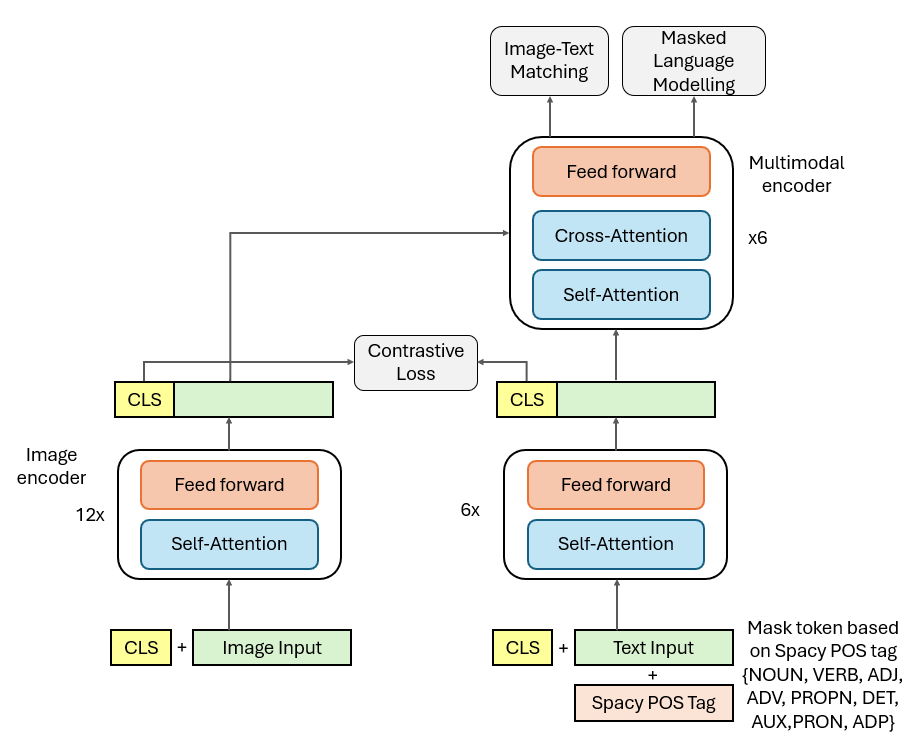
\includegraphics[width=0.6\textwidth]{Images/overview.png}
    \end{center}
    \small
\end{figure}

\section{Model architecture}
As shown in Figure \ref{fig:overview}, our model include with 3 main component, an image encoder, a text encoder and a multimodal encoder. 
The first one is image encoder, which we used ResNet \cite{resnet} architecture and modified following OpenClip as a image encoder in this experiment.
The second one is text encoder, which used transformer architecture as BERT \cite{bert} to encode image caption.
The last one is multimodal encoder.
This part is where \acrshort{vl} interaction is occurs.
Given a training dataset \(D\) consisting of image-text pairs \((v_i, t_i) \in D\), where \(v_i\) is the image and \(t_i\) is the image caption of the \(i\)-th image, 
The image encoder


\section{Mask language modelling}
Our model is trained with the \acrshort{mlm} task.
Normally, a percentage of tokens \(\{w_1,...w_T\}\) are replaced with a special [MASK] token to create a masked caption \(t_i^{\text{mask}}\).
However, in this work, the masked tokens are based on the type of \acrshort{pos} instead of randomly masking.
The model is then trained to predict the original tokens at the masked positions, conditioned on both the unmasked tokens in \(t_i^{\text{mask}}\) and the visual features of \(v_i\). 

Formally, let \(M\) be the set of positions in \(t_i\) where tokens have been masked. 
The model’s objective is to maximize the probability of the original tokens at these masked positions, given by:
\[
\mathcal{L}_{\text{MLM}} = - \sum_{m \in M} \log P\left(t_i[m] \mid t_i^{\text{mask}}, v_i\right),
\]
where \(t_i[m]\) is the original token at position \(m\) in \(t_i\), and \(P(t_i[m] \mid t_i^{\text{mask}}, v_i)\) is the model's predicted probability of the token based on both the masked caption and the visual context. 

% \subsection{Mask langauge modelling}

% \subsection{Image-text contrative learning}

% \subsection{Image-text matching}
\section{Part of speech tagging}


\section{Dataset}


\section{Visual question answering}


\section{Implementation Detail}
BF16 datatype